%Beamer class
\documentclass{beamer}

\usepackage[czech]{babel}
\usepackage[cp1250]{inputenc}
\usepackage{fontenc}
\usepackage{tgheros}
\usepackage{array}
\usepackage{color}
\usepackage{hyperref}

\usetheme{Antibes}
\usecolortheme{crane}


\title[BE1M13VES]{BE1M13VES}
\subtitle[Manufacturing of Electrical Components] {Manufacturing of Electrical Components}
\author[Brejcha]{Michal Brejcha}
\institute[CTU]{CTU in Prague}
\date[Prague, 2017]{Prague, 2017}

\begin{document}
%------------------------------------------------------------------------------
%Uvodni slajd
%------------------------------------------------------------------------------
\frame{\titlepage}

\begin{frame}
\frametitle{Overview} 
\tableofcontents
\end{frame}

\AtBeginSection[]
{
  \begin{frame}
    \frametitle{TOPIC}
    \tableofcontents[currentsection]
  \end{frame}
}

%------------------------------------------------------------------------------
%Resistance value
%------------------------------------------------------------------------------
\section{\texorpdfstring{Resistance value}{Resistance value}}
%------------------------------------------------------------------------------
	\begin{frame}
    \frametitle{Resistors}
		\begin{center}
		\begin{tabular}{p{0.3\linewidth} p{0.6\linewidth}}
			\textbf{Parameters:} 					& 
			\begin{itemize}
				\item $R$... electric resistance,
				\item $\delta$... value tolerance,
				\item $P_{max}$... dissipated power,
				\item $TCR$... temperature coefficient of resistivity,
				\item $VCR$, $THI$... voltage dependence of rezistivity,
				\item frequency dependence,
				\item noise, non-linearity ($THI$), aging.
			\end{itemize}
			\\

		\end{tabular}
		\end{center}
  \end{frame}
%------------------------------------------------------------------------------
	\begin{frame}
    \frametitle{Resistivity}
		\begin{center}
		\begin{tabular}{p{0.4\linewidth} p{0.5\linewidth}}
			\textbf{Resistance of a wire:} 					& $$R = \rho\cdot\frac{l}{S}$$\\
		\end{tabular}
		\begin{tabular}{p{0.1\linewidth} p{0.8\linewidth}}
			$\rho$...																& resistivity in $\Omega m$ or $\Omega mm^2/m$\\
			$l$...																	& wire length in $m$\\
			$S$...																	& surface area in $m^2$ or $mm^2$\\
		\end{tabular}
			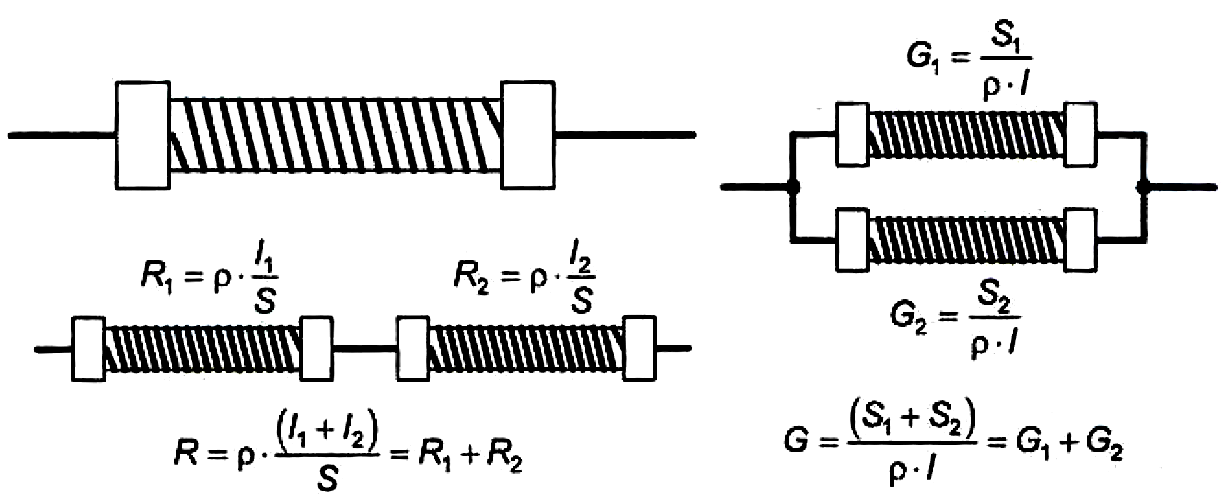
\includegraphics[scale=0.25]{obr01_spojovaniR.png}
		\end{center}
  \end{frame}
%------------------------------------------------------------------------------
	\begin{frame}
    \frametitle{Normalization - Geometric Progression}
		\begin{center}
		\begin{tabular}{p{0.2\linewidth} p{0.7\linewidth}}
			\textbf{Marking:} 					& $E6$, $E12$, $E24$,..., $EX$\\\\
			$E$...											& geometric (exponential) sequence,\\
			$X$...											& count of values per decade, \\
																	& $X = 3\cdot 2^n$, $n=1,2,3,...$\\\\
			\textbf{Base value:}				& $$b= \sqrt[X]{10}$$\\
			\textbf{Precision:}					& $$\delta\approx \frac{100}{X}\%$$
		\end{tabular}
		\end{center}
  \end{frame}
%------------------------------------------------------------------------------
	\begin{frame}
    \frametitle{E6, E12, E24}
		\begin{center}
		\begin{tabular}{c}
		$E6 = (b^0, b^1,...,b^5)\cdot 10^E = 1.00, 1.47, 2.15,...,6.81$\\\\
		\end{tabular}

		\begin{tabular}{|l |c c c c c c|}
			\hline
			E6 &1.0 &1.5 &2.2 &3.3 &4.7 &6.8\\
			$\delta = 20\%$ &&&&&&\\
			\hline
			E12 &1.0 &1.2 &1.5 &1.8 &2.2 &2.7\\
			$\delta = 10\%$&3.3 &3.9 &4.7 &5.6 &6.8 &8.2\\
			\hline
			E24 &1.0 &1.1 &1.2 &1.3 &1.5 &1.6\\
			$\delta = 5\%$	&1.8 &2.0 &2.2 &2.4 &2.7 &3.0\\ 
					&3.3 &3.6 &3.9 &4.3 &4.7 &5.1\\
					&5.6 &6.2 &6.8 &7.5 &8.2 &9.1\\
			\hline
		\end{tabular}
		\end{center}
  \end{frame}
%------------------------------------------------------------------------------
	\begin{frame}
    \frametitle{Tolerance boundaries approximation}
		\begin{center}
		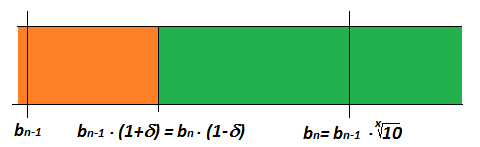
\includegraphics[scale=0.65]{obr02_tolerancniPasma.png}
		$$1+\delta = \sqrt[X]{10}\cdot (1-\delta)$$
		$$\delta = \frac{\sqrt[X]{10} - 1}{\sqrt[X]{10} + 1}$$
		Consider $X > 6$, then $\sqrt[X]{10} \rightarrow 1$ and $\frac{\partial\delta}{\partial X} \approx \frac{\partial}{\partial X}\left(\frac{1}{X}\right)$
		$$\delta \approx \frac{1}{X}$$
		
		\end{center}
  \end{frame}
%------------------------------------------------------------------------------
	\begin{frame}
    \frametitle{Component Identification}
		\begin{center}
		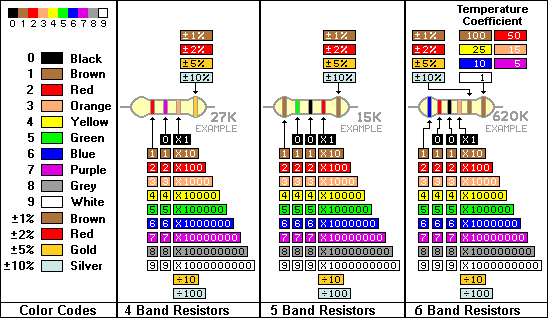
\includegraphics[scale=0.65]{obr03_barevneZn.png}\\
		\begin{tabular}{p{0.1\linewidth} p{0.8\linewidth}}
			\tiny{\textbf{Source:}} 	& \tiny{\url{www.diyaudioandvideo.com/Electronics/ResistorColorCodes/}}\\
		\end{tabular}
		\end{center}
  \end{frame}
%------------------------------------------------------------------------------
	\begin{frame}
    \frametitle{Component Identification - OLD or for Power Resistors}
		\begin{center}
		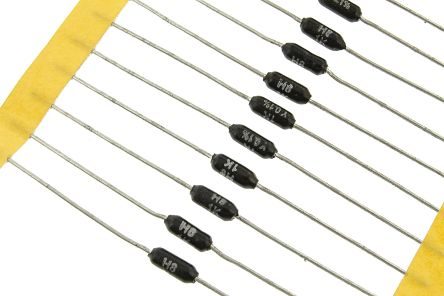
\includegraphics[scale=0.4]{obr04_vykonoveZn.png}\\
		\begin{tabular}{p{0.1\linewidth} p{0.8\linewidth}}
			\tiny{\textbf{Source:}} 	& \tiny{\url{uk.rs-online.com/web/p/through-hole-fixed-resistors/7017383/}}\\
		\end{tabular}
		\begin{description}
		\item[Value:] 2 or 3 first digits. Sometimes $R$ is used as symbol for the radix point.
		\item[Multiplier:] \textbf{R}=~$10^0$, \textbf{k}=~kilo=~$10^3$, \textbf{M}=~mega=~$10^6$, \textbf{G}=~giga=~$10^6$\\
											It works as radix point
		\item[Tolerance:]	2 digits with $\%$ symbol
		\end{description}
		\end{center}
  \end{frame}
%------------------------------------------------------------------------------
	\begin{frame}
    \frametitle{Component Identification - SMT (SMD)}
		\begin{center}
		\begin{tabular}{p{0.2\linewidth} p{0.3\linewidth}}
				3 digits:& $\delta> 1\%$\\
				4 digits:& $\delta< 1\%$\\\\
				Example: & $30R9\rightarrow 30.9 \Omega$, \\
								 & $\delta< 1\%$\\
								 & $391\rightarrow 390 \Omega$\\
								 & $270\rightarrow 27 \Omega$\\
		\end{tabular}
		\begin{tabular}{p{0.3\linewidth}}
			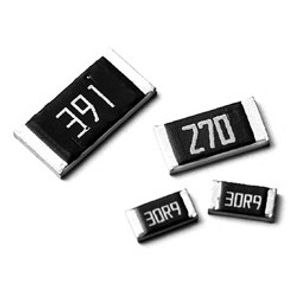
\includegraphics[scale=0.35]{obr05_smdZn.png}\\
			\tiny{\textbf{Source: }\url{gme.cz}}\\
		\end{tabular}
		
		\begin{description}
		\item[Value:] 2 or 3 first digits.
		\item[Multiplier:] It is the last digit whenever $R$ symbol missing $\Rightarrow$ power of 10.\\
											 For small values $R$ symbol replacing the radix point.
		\end{description}

		\end{center}
  \end{frame}
%------------------------------------------------------------------------------
%Design
%------------------------------------------------------------------------------
\section{\texorpdfstring{Technology}{Technology}}
%------------------------------------------------------------------------------
	\begin{frame}
    \frametitle{Technology Overview}
		\begin{center}
		\begin{tabular}{p{0.35\linewidth} p{0.55\linewidth}}
			\textbf{Film resistors:} 	& carbon, metal, metal-oxide layer; They are most common in electronics\\
			\textbf{Varnished resistors:} 	& varnished-carbon film, just for high voltage appl.\\
			\textbf{Wire resistors:} 	& power dumping resistor, variable resistors.\\
		\end{tabular}
		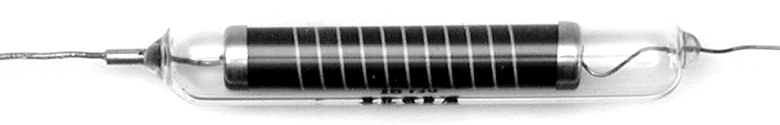
\includegraphics[scale=0.3]{obr06_vrstvovyRez.png}
		\end{center}
		\textbf{Value precise setting:}\\
		\begin{tabular}{p{0.35\linewidth} p{0.55\linewidth}}
			\textbf{Film resistors:} 	& via spiral trace in the layer,\\
			\textbf{Wire resistors:} 	& via length of the wire.\\
		\end{tabular}
  \end{frame}
%------------------------------------------------------------------------------
	\begin{frame}
    \frametitle{Technology - Film Resistors}
		\begin{center}
		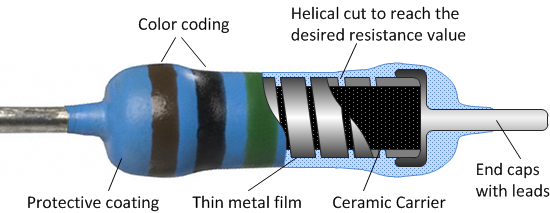
\includegraphics[scale=0.4]{obr07_sroubovice.png}\\
		\tiny{\textbf{Source: }\url{www.resistorguide.com/pictures/metal_film_resistor_schematic.png}}\\
		\end{center}
		\textbf{Carbon resistors}
		\begin{itemize}
			\item \small{Device is made of ceramic cylinder body (e.g. alkalic ceramic) and covered with carbon layer. Layer of carbon is made by heat decompositions of some hydrocarbon (e.g. $CH_2-CH_2$).}
		\end{itemize}
		
		\textbf{Metal resistors}
		\begin{itemize}
			\item \small{Design is similar to carbon resistors. Layer with required resistivity is made from some metal - typically from chrome-nickel alloy ($Cr-Ni$) or $Si-Fe-Cr$.}
		\end{itemize}
  \end{frame}
%------------------------------------------------------------------------------
	\begin{frame}
    \frametitle{Technology - Film Resistors}
		\textbf{Metal-oxide resistors (MOX)}
		\begin{itemize}
			\item Design is similar to metal and carbon resistors. Layer with resistivity is made from $SnO_2$ by using of  reactive (jet) vapor deposition.
		\end{itemize}
		
		\textbf{Varnished (lacquered) resistors}
		\begin{itemize}
			\item Resistive layer is sprayed on a ceramic body. Layer consist from polymer binder (varnish - terephthalate), resistivity is managed by graphite filler (soot). Layer have a huge specific resistivity!
		\end{itemize}
  \end{frame}
%------------------------------------------------------------------------------
	\begin{frame}
    \frametitle{Thick ant Thin Film Resistors - SMT}
		\textbf{Thick-layer resistors}
		\begin{itemize}
			\item In the past these resistors were used in hybrid devices (printed circuit board on ceramic plate with integrated semiconductor part. Today's some of thick layer resistors are made and used for surface mounted technology (SMT).  Features are similar to layer metal and metal-oxide resistors.
		\end{itemize}
		
		\textbf{Thin-layer resistors}
		\begin{itemize}
			\item Big specific resistivity on square of thin layer is suitable for thin-layer resistors. Also such layer can exhibit low $TCR$ (lower than $10^{-4}$ K$^{-1}$) The layer is made by vapor deposition on smooth and flat basis - glass, ceramic. Typical shape of such resistor is a meander or strip.
		\end{itemize}
  \end{frame}
%------------------------------------------------------------------------------
	\begin{frame}
    \frametitle{Thick ant Thin Film Resistors - SMT}
		\begin{center}
		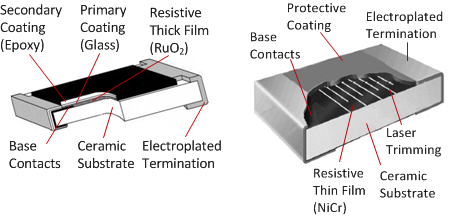
\includegraphics[scale=0.5]{obr08_tlusteTenke.png}\\
		\tiny{\textbf{Source: }\url{www.resistorguide.com/thin-and-thick-film/}}\\
		\end{center}
		\begin{center}
		\begin{tabular}{p{0.3\linewidth} | c | c}
			\hline
			\textbf{Parameter} 					& \textbf{Thick} 	& \textbf{Thin}\\
			\hline
			Values ($\Omega$) 					& $1 - 100$M    	& $0.2 - 20$M\\
			\hline
			Tolerance ($\%$) 	  				&$\pm 1 - \pm 5$ 	& $\pm 0.1 - \pm 2$ \\
			\hline
			TCR ($K^{-1}$) 	  					&$(5 - 20)\cdot 10^{-5}$ 			& $(5 - 50)\cdot 10^{-6}$ \\
			\hline
			1000 h stability ($\%$) 	  &$\pm 1 - \pm 3$ 			& $\pm 0.15 - \pm 0.5$  \\
			\hline
		\end{tabular}
		\end{center}
  \end{frame}
%------------------------------------------------------------------------------
	\begin{frame}
    \frametitle{Wire Resistors}
		\textbf{Power Resistors}
		\begin{itemize}
			\item Coiled ceramic body with resistive wire. Chrome-nickel wire is used for applications at high temperature (e.g. $350^\circ$C). The winding is made only in one layer and the insulation is got from oxide layer on wires. 
		\end{itemize}
		
		\textbf{Precise Resistors}
		\begin{itemize}
			\item They are not dedicated and used for power application nor for high temperature operation. Resistors consist from ceramic or plastic body and from multi-layer winding. Winding is made from isolated Manganin, Kanthal or Constantan wire. Low TCR is required!
		\end{itemize}
		\textbf{\color{red}{coil $\Rightarrow$ large parasitic inductance}}
  \end{frame}
%------------------------------------------------------------------------------
	\begin{frame}
    \frametitle{Winding}
		\begin{center}
		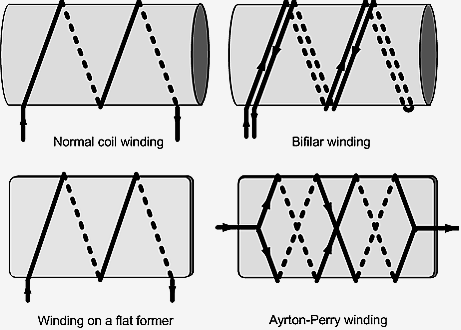
\includegraphics[scale=0.7]{obr09_vinuti.png}\\
		\end{center}
  \end{frame}
%------------------------------------------------------------------------------
%Parasitic parameters
%------------------------------------------------------------------------------
\section{\texorpdfstring{Parasitic Parameters}{Parasitic Parameters}}
%------------------------------------------------------------------------------
	\begin{frame}
    \frametitle{Temperature Dependency of Resistivity}
		\begin{itemize}
			\item TCR - Temperature Coefficient of Resistivity. 
			\item clean metals (not contaminated) \textbf{TCR}: $(2-10)\cdot 10^{-3}$ K$^{-1}$, \\ \color{blue}{($Fe - 10$; $W$, $Mo - 5.5$; $Cu - 4$; $Pt - 3.8$)}\\
			\item \color{black}{alloys exhibit lower \textbf{TCR}:}\\ \color{blue}{brass ($Cu + Zn$) $- 1.5\cdot 10^{-3}$ K$^{-1}$}\\
			\item \color{black}{resistive alloys have the lowest \textbf{TCR}:}\\ $(1-3)\cdot 10^{-5}$ K$^{-1}$\color{blue}{(Manganin, Constantan)}
		\end{itemize}
		\textbf{Dependency can be approximated by:}
		$$R = R_0\cdot \left(1+TCR\cdot \left(T-T_0\right)\right)$$
  \end{frame}
%------------------------------------------------------------------------------
	\begin{frame}
    \frametitle{Voltage Dependency of Resistivity}
		\begin{itemize}
			\item VCR - Voltage Coefficient of Resistivity - \textbf{NONLINEARITY}. 
			\item Under voltage stress (voltage loading) can be at maximum up to $10\%$ of nominal resistivity (bulk, varnished resistors). Linear resistors (metal, metal-oxide) - low dependence (VCR $< 10^{-6}$ V$^-1$).

		\end{itemize}
		\textbf{Dependency can be approximated by:}
		$$R = R_0\cdot \left(1+VCR\cdot \left(U-U_0\right)\right)$$
		$$VCR = \frac{R-R_0}{\left(U-U_0\right)\cdot R_0}$$
  \end{frame}
%------------------------------------------------------------------------------
	\begin{frame}
    \frametitle{Noise}
		\textbf{Thermal noise}
		\begin{itemize}
			\item Thermal noise is a non-periodic, non-harmonic random signal with natural origin. It is frequency independent. 
		\end{itemize}
		$$U_n^2= 4\cdot k\cdot T\cdot B\cdot R$$
		\small{$U_n$ is an average noise voltage; \\ $k$ is a Boltzmann's const. $1.38\cdot 10^{-23}$ J$/$K; \\ $T$ is absolute temperature; \\ $B$ is equivalent frequency bandwidth; \\ $R$ is a resistivity. }

  \end{frame}
%------------------------------------------------------------------------------
	\begin{frame}
    \frametitle{Noise}
		\textbf{Current noise}
		\begin{itemize}
			\item The level of current noise is critical especially in low-frequency audio and video HiFi devices. Current noise is a quality marker and can be used for predictions of reliability and life-time of devices. It is frequency dependent.
		\end{itemize}
		$$u_n^2(f)= \frac{A\cdot I^\alpha\cdot R^\beta}{f}$$
		\small{$u_n^2$ is a square of noise voltage measured in 1Hz band,\\ $A$ is a quality marker of used resistor,\\ $I$ is a load current,\\ $f$ is a frequency,\\ $\alpha$, $\beta$ are parameters depending on the type of resistor (typically $\alpha = \beta = 2$).}

  \end{frame}
%------------------------------------------------------------------------------
	\begin{frame}
    \frametitle{Total noise}
		\begin{center}
		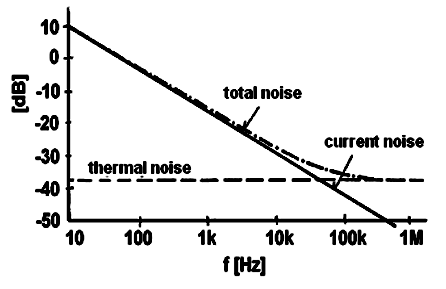
\includegraphics[scale=0.7]{obr10_sum.png}\\
		\end{center}
  \end{frame}
%------------------------------------------------------------------------------
\end{document}